\documentclass[12pt]{article}
\input{bayesuvius.sty}



\begin{document}
\title{Causal DAG for genes obtained via Mappa Mundi algorithm}
\date{ \today}
\author{Robert R. Tucci\\
        tucci@ar-tiste.com}
\maketitle
\vskip2cm
\section*{Abstract}

\section{Introduction}

This paper can be viewed
as an application and further refinement 
of the Mappa Mundi (MM) algorithm.  
In this case, we apply it to finding what
are called Gene Regulatory Networks (GRN)
and Network Motifs 
in the Genomics and Systems Biology literature (Ref.\cite{alon-book}).


The MM algorithm
was first proposed in Ref.\cite{mappa-mundi} 
for DAG Extraction From Text (DEFT). 
In Ref.\cite{mappa-mundi}, it was used to compare 3 P.G. Wodehouse short stories and the scripts of 3 PiXar movies
and extract from those causal DAGs.
In general, the MM algorithm can extract causal DAGs from 2 or more 
text files, as long as each of
those text files recounts actions 
in chronological order. So it will work with time stamped lab
notebooks or medical records, 
but it won't work with textbooks or fiction with  time travel or flashback shenanigans.

After Ref.\cite{mappa-mundi}, the MM algorithm was later applied in Ref.\cite{causal-fitbit} to extracting causal DAGs from FitBit times
series data.

In this paper, we use the MM algorithm
to extract DAGs from time series data for
concentrations of
gene expressions and transcription factors.
The DAGs we obtain are called GRN
in the Genomics literature. GRN are a
special case of autoregulon networks.

Autoregulons Networks (AN) are 
discussed in the chapter entitled \qt{Autoregulon Networks (Network Motifs)} of 
my book Ref.\cite{Bayesuvius}.

AN are a special case of Dynamical systems (DS). DS are discussed in the
chapter entitled \qt{Dynamical Systems}
of my book Ref.\cite{Bayesuvius}.


\section{Comparing 2 TS Records}
\begin{figure}[h!]
\centering
\includegraphics[width=5in]
{two-phase-plane-bridges.png}
\caption{Causal bridges $a$ and $b$ spanning
	phase planes for
TS records 1 and 2.}
\label{fig-two-phase-plane-bridges}
\end{figure}

We will use the term {\bf time series (TS) record}
to refer to
a data file such as a spreadsheet with the first column 
giving time increasing downwards and additional column giving the values
of $q_i$ (a state variable) and $\dot{q}_i$ (time derivative of $q_i$) for $i=1, 2, \ldots N$
at the time indicated by the first column.
Any $q_i$ or $\dot{q}_i$ is called a {\bf state variable}.
The multidimensional space $(q_i)_{i=0}^{N}$
is called {\bf configuration space}
The multidimensional space $(q_i, \dot{q}_i)_{i=0}^{N}$
is called {\bf phase space}.
A two dimensional space $(q_i, \dot{q}_i)$ for any 
$i$ is called a {\bf phase plane}.

The TS record may contain initially only a column 
for time and columns for configuration space,
if the change in time between rows is small. 
In that case we can subtract two consecutive
$q_i$ readings and divide by the difference
in times to obtain the $\dot{q}_i$ column
and same row.

For this paper, each $q_i$ represents either a {\bf translation
factor (TF)} concentration, or a {\bf gene expression (GE)} concentration.\footnote{The 
terms \qt{translation factor}
and \qt{gene expression} are both defined
in the AN chapter of my free book Ref.\cite{Bayesuvius}}


Suppose $x$ annd $y$
are any two $q_i$. For $\xi \in\{x\rarrow y, y\rarrow x\}$, let

$n_{acc}^{\xi}$: number of arrows , initially zero

$n_{rej}^{\xi}$: number of arrows rejected, initially zero

$N^{\xi}=n_{acc}^\xi+ n_{rej}^\xi$: number of arrows detected

$p_{acc}^{\xi}=\frac{n_{acc}^{\xi}}
{n_{acc}^{\xi}+n_{rej}^{\xi}}$: probability of causal arrow, initially zero.

$N^*$: threshold value for
$N^\xi$

$p_{acc}^*$: threshold value for 
$p_{acc}^\xi$

The MM algorithm 
for finding an AN 
from 2 TS records, consists of the following steps:
\begin{enumerate}
\item {\bf Compare 2 TS records
and score arrows between any two  autoregulons
nodes $\boxed{\rvx}$ and 
$\boxed{\rvy}$}


Consider Fig.\ref{fig-two-phase-plane-bridges}.
In that figure, suppose the two ends of bridge $a$ are equal: $\calx_1(t_a)\approx \calx_2(t_a')$ and
the two ends of bridge $b$ are equal too:
$\caly_1(t_b)\approx \caly_2(t_b')$. \footnote{By $\calx\approx \caly$ we mean that both of these vectors are inside the same small bin or open ball
of size given by a pre-specified precision.}

At the very least, 
one must store
(unless they are  the default value zero) the current values
 of $n_{acc}^\xi$ and $n_{rec}^\xi$ 
for $\xi \in\{x\rarrow y, y\rarrow x\}=\cala$, where $x$ and $y$ are any two $q_i$. 


\begin{itemize}

\item if $t_a<t_b$ and $t_a'<t_b'$ (bridges are parallel in time)\footnote{$x++$ means add 1 to $x$}

\beq
\left\{
\begin{array}{l}
n_{acc}^{x\rarrow y}++
\\
N^{x\rarrow y}++
\end{array}
\right.
\eeq

\item if $t_a>t_b$ and $t_a'>t_b'$ (bridges are parallel in time)

\beq
\left\{
\begin{array}{l}
	n_{acc}^{y\rarrow x}++
	\\
	N^{y\rarrow x}++
\end{array}
\right.
\eeq

\item if $t_a<t_b$ and $t_a'>t_b'$ (bridges are crossing in time)

\beq
\left\{
\begin{array}{l}
	n_{rej}^{x\rarrow y}++
	\\
	N^{x\rarrow y}++
\end{array}
\right.
\eeq

\item if $t_a>t_b$ and $t_a'<t_b'$ (bridges are crossing in time)

\beq
\left\{
\begin{array}{l}
	n_{rej}^{y\rarrow x}++
	\\
	N^{y\rarrow x}++
\end{array}
\right.
\eeq
\end {itemize}

\item {\bf Draw DAG}

\beq
\xymatrix@C=10pc{
\Rect{\rvx}\ar@{->}@/_1pc/[r]|{p_{acc}^{x\rarrow y}(N^{x\rarrow y})}
\ar@{<-}@/^1pc/[r]|{p_{acc}^{y\rarrow x}(N^{y\rarrow x})}
&\Rect{\rvy}
}
\label{eq-x-y-autos}
\eeq
If $x$ and $y$ are any two
$q_i$, draw an arrow from autoregulon $\boxed{\rvx}$
to autoregulon $\boxed{\rvx}$
iff both $p_{acc}^{x\rarrow y}>p^*$
and $N^{x\rarrow y}> N^*$
are true.


Likewise,
draw an arrow from autoregulon $\boxed{\rvy}$
to autoregulon $\boxed{\rvx}$
iff both $p_{acc}^{y\rarrow x}>p^*$
and $N^{y\rarrow x}> N^*$
are true.

When drawing an arrow, put 
the values $p_{acc}^\xi$ and
$N^\xi$ over the arrow, where 
$\xi\in\cala$. See Eq.(\ref{eq-x-y-autos})
where this is done with variables. Do it with the values of those variables instead.

At first glance, 
Eq.(\ref{eq-x-y-autos}) doesn't look like a DAG, because it has a cycle and DAGs are, by definition, acyclic. But
Eq.(\ref{eq-x-y-autos}) does indeed represent a DAG because, as explained
in the AN chapter of Ref.\cite{Bayesuvius},
Eq.(\ref{eq-x-y-autos})
represents this net: 

\beq
\xymatrix{
\rvx \ar[d]\ar[dr]
& \rvy\ar[d]\ar[dl]
\\
\dot{\rvx} & \dot{\rvy}
}
\eeq


which is acyclic.





\end{enumerate}

\section{Comparing More Than 2 TS Records}

\bibliographystyle{plain}
\bibliography{references}
\end{document}



